\chapter{Inflação}
\label{les:9}

\begin{chapquote}{A Rainha de Copas} % TODO: check if it's the queen or not
\enquote{Agora, aqui, sabe, é necessário toda a corrida que você tem para se manter no mesmo lugar. Se você quer ir a um lugar diferente, você deve correr pelo menos duas vezes mais rápido que aquilo!}
\end{chapquote}

Tentar entender a inflação monetária e como um sistema não inflacionário como o Bitcoin pode mudar a forma como fazemos as coisas foi o ponto de partida de minha aventura em economia. Eu sabia que a inflação era a taxa pela qual o dinheiro novo era criado, mas não sabia muito além disso.

Enquanto alguns economistas argumentam que a inflação é uma coisa boa, outros argumentam que o dinheiro \enquote{forte}, que não pode ser inflado facilmente --- como tínhamos na época do padrão ouro --- é essencial para uma economia saudável. O Bitcoin, com seu suprimento fixo de 21 milhões, concorda com o último argumento.

Normalmente, os efeitos da inflação não são imediatamente óbvios. Dependendo da taxa de inflação (bem como de outros fatores), o tempo entre a causa e o efeito pode ser de vários anos. Não só isso, mas a inflação afeta diferentes grupos de pessoas de formas diferentes. Como Henry Hazlitt aponta em \textit{Economia em Uma Lição}: \enquote{A arte da economia consiste em olhar não apenas para o imediato, mas para os efeitos de longo prazo de qualquer ato ou política; consiste em rastrear as consequências dessa política não apenas para um grupo, mas para todos eles.}

Um dos meus momentos de iluminação pessoal foi a percepção de que emitir moeda --- imprimir mais dinheiro --- é uma atividade econômica \textit{completamente} diferente de todas as outras atividades econômicas. Enquanto bens e serviços reais produzem valor real para pessoas reais, imprimir dinheiro efetivamente faz o oposto disso. Diminui o valor de todos os que detêm a moeda que está sendo inflacionada.

\begin{quotation}\begin{samepage}
\enquote{Mera inflação --- isto é, a mera emissão de mais dinheiro, com a consequência de maiores salários e preços --- pode parecer a criação de maior demanda. Mas, em termos de produção e trocas reais de coisas reais, não é.}
\begin{flushright} -- Henry Hazlitt\footnote{Henry Hazlitt, \textit{Economia em Uma Lição} \cite{hazlitt}}
\end{flushright}\end{samepage}\end{quotation}

A força destrutiva da inflação torna-se óbvia assim que um pouco de inflação se transforma em \textit{muita}. Se a moeda chega a ser hiperinflada, as coisas ficam feias rapidamente. \footnote{\url{https://en.wikipedia.org/wiki/Hyperinflation} \cite{wiki:hyperinflation}} Conforme o poder de compra da moeda inflacionada se desfaz, ela deixará de armazenar valor com o tempo, com isso as pessoas correrão para colocar seu dinheiro em bens que possam servir como reserva de valor.

\paragraph{}
Outra consequência da hiperinflação é que todo o dinheiro que as pessoas economizaram ao longo da vida efetivamente desaparecerá. O papel-moeda dentro de nossa carteira ainda estará lá, é claro. Mas será exatamente isso: papel sem valor.

\begin{figure}
  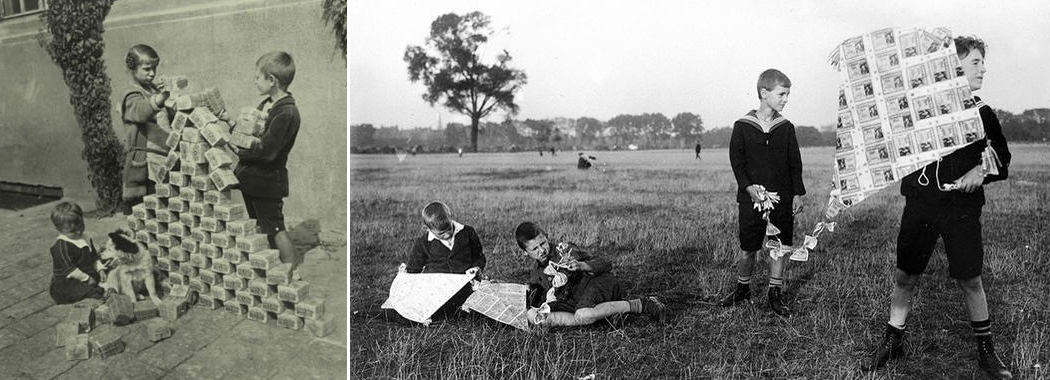
\includegraphics{assets/images/children-playing-with-money.png}
  \caption{Hiperinflação na República de Weimar (1921-1923)}
  \label{fig:children-playing-with-money}
\end{figure}

\paragraph{}
O dinheiro também perde valor com a chamada inflação \enquote{moderada}. Simplesmente acontece devagar o suficiente para que a maioria das pessoas não perceba a diminuição do seu poder de compra. E uma vez que as impressoras estão funcionando, a moeda pode ser facilmente inflada, e o que costumava ser uma inflação branda pode se transformar em uma dolorosa inflação descontrolada com o apertar de um botão. Como Friedrich Hayek apontou em um de seus ensaios, a inflação branda geralmente leva à inflação total.

\begin{quotation}\begin{samepage}
\enquote{A inflação `moderada' e suave não pode ajudar --- ela só leva a uma inflação absoluta.}
\begin{flushright} -- Friedrich Hayek\footnote{Friedrich Hayek, \textit{1980s
Desemprego e Sindicatos} \cite{hayek-inflation}}
\end{flushright}\end{samepage}\end{quotation}

A inflação é particularmente maléfica, pois favorece aqueles que estão mais próximos das impressoras. Leva tempo para que o dinheiro recém-criado circule e os preços se ajustem, portanto se você conseguir colocar as mãos em mais dinheiro antes que o todo mundo se desvalorize, você estará à frente da curva inflacionária. É também por isso que a inflação pode ser vista como um imposto disfarçado porque no final os governos lucram com isso enquanto todos os outros acabam pagando o preço.

\begin{quotation}\begin{samepage}
\enquote{Não acho exagero dizer que a história é, em grande parte, uma história de inflação e, geralmente, de inflações criadas por governos para ganhos dos próprios governos.}
\begin{flushright} -- Friedrich Hayek\footnote{Friedrich Hayek, \textit{O Bom Dinheiro} \cite{hayek-good-money}}
\end{flushright}\end{samepage}\end{quotation}

Até agora, todas as moedas controladas pelo governo foram eventualmente substituídas ou entraram em colapso total. Não importa quão pequena seja a taxa de inflação, crescimento \enquote{estável} é apenas outra maneira de dizer crescimento exponencial. Na natureza, assim como na economia, todos os sistemas que crescem exponencialmente terão que se estabilizar ou sofrer um colapso catastrófico.

\paragraph{}
\enquote{Isso não vai acontecer no meu país}, é o que você provavelmente está pensando. Você não pensaria isso se você fosse da Venezuela, que atualmente está sofrendo com a hiperinflação. Com uma taxa de inflação de mais de um milhão por cento, o dinheiro é praticamente inútil. \cite{wiki:venezuela}

\paragraph{}
Isso pode não acontecer nos próximos anos ou com a moeda específica usada em seu país. Mas dê uma olhada na lista de moedas históricas \footnote{Veja \textit{Lista de moedas históricas} na Wikipedia. \cite{wiki:historical-currencies}} que mostra que isso inevitavelmente acontecerá no longo prazo. Eu me lembro de usar muitas das moedas listadas: o xelim austríaco, o marco alemão, a lira italiana, o franco francês, a libra irlandesa, o dinar croata, etc. Minha avó até usava a coroa austro-húngara. Conforme o tempo passa, as moedas atualmente em uso \footnote{Veja \textit{Lista de moedas} na Wikipedia \cite{wiki:list-of-currencies}} irão caminhar lentamente, mas seguramente, para seus respectivos cemitérios. Eles irão hiperinflacionar ou serão substituídas. Em breve, serão moedas históricas. Vamos torná-las obsoletas.

\begin{quotation}\begin{samepage}
\enquote{A história tem nos mostrado que os governos inevitavelmente sucumbirão ao
tentação de inflar a oferta de dinheiro.}
\begin{flushright} -- Saifedean Ammous\footnote{Saifedean Ammous, \textit{O Padrão Bitcoin} \cite{bitcoin-standard}}
\end{flushright}\end{samepage}\end{quotation}

\newpage

Por que o Bitcoin é diferente? Em contraste com as moedas dos governos, bens monetários que não são regulamentados pelos Estados, mas pelas leis da física \footnote{Gigi, \textit{Consumo de energia do Bitcoin - Uma mudança de perspectiva} \cite {gigi:energy}}, tendem a sobreviver e até manter valor ao longo do tempo. O melhor exemplo disso até agora é o ouro, que conforme o apropriadamente denominado \textit{Gold-to-Decent-Suit Ratio} \footnote{A história mostra que o preço de uma onça de ouro é igual ao preço de um terno masculino decente de acordo com os gerentes de investimento da Sionna \cite{web:gold-to-decent-suite-ratio}} mostra, está mantendo seu valor por centenas e até milhares de anos. Pode não ser perfeitamente \enquote{estável} --- um conceito questionável em primeiro lugar --- mas o valor que ele possui será, pelo menos, da mesma ordem de magnitude.

Se um bem monetário ou moeda mantém bem seu valor ao longo do tempo e do espaço, ele é considerado \textit{forte}. Se não consegue manter o seu valor, porque se deteriora ou infla facilmente, é considerada uma moeda \textit{fraca}. O conceito de força é essencial para entender o Bitcoin e merece um exame mais aprofundado. Voltaremos a falar dele na última lição econômica: O dinheiro forte.

\paragraph{}
À medida que mais e mais países sofrem com a hiperinflação, mais e mais pessoas terão que enfrentar a realidade do dinheiro forte e fraco. Se tivermos sorte, talvez até mesmo alguns banqueiros centrais sejam forçados a reavaliar suas políticas monetárias. Aconteça o que acontecer, as percepções que ganhei graças ao Bitcoin provavelmente serão inestimáveis, não importa o resultado.

\paragraph{O Bitcoin me ensinou sobre como a inflação é um imposto disfarçado e a catástrofe da hiperinflação.}

% ---
%
% #### Down the Rabbit Hole
%
% - [Economics in One Lesson][Henry Hazlitt] by Henry Hazlitt
% - [1980's Unemployment and the Unions][unions] by Friedrich Hayek
% - [Good Money, Part II][good-money]: Volume Six of the Collected Works of F.A. Hayek
% - [The Bitcoin Standard] by Saifedean Ammous
% - [Hyperinflation][hyperinflates], [economic crisis in Venezuela][wiki-venezuela], [list of historical currencies], [list of currencies][currently in use] on Wikipedia
%
% [unions]: https://books.google.com/books/about/1980s_unemployment_and_the_unions.html?id=xM9CAQAAIAAJ
% [good-money]: https://books.google.com/books?id=l_A1vVIaYBYC
%
% [Henry Hazlitt]: https://mises.org/library/economics-one-lesson
% [hyperinflates]: https://en.wikipedia.org/wiki/Hyperinflation
% [inflation cannot help]: https://books.google.com/books?id=zZu3AAAAIAAJ&dq=%22only+while+it+accelerates%22&focus=searchwithinvolume&q=%22steady+inflation+cannot+help%22
% [history of inflation]: https://books.google.com/books?id=l_A1vVIaYBYC&pg=PA142&dq=%22history+is+largely+a+history+of+inflation%22&hl=en&sa=X&ved=0ahUKEwi90NDLrdnfAhUprVkKHUx1CmIQ6AEIKjAA#v=onepage&q=%22history%20is%20largely%20a%20history%20of%20inflation%22&f=false
% [wiki-venezuela]: https://en.wikipedia.org/wiki/Crisis_in_Venezuela#Economic_crisis
% [by the laws of physics]: https://link.medium.com/9fzq2L0J3S
% [\textit{Gold-to-Decent-Suit Ratio}]: https://www.businesswire.com/news/home/20110819005774/en/History-Shows-Price-Ounce-Gold-Equals-Price
% [The Bitcoin Standard]: https://thesaifhouse.wordpress.com/book/
%
% <!-- Wikipedia -->
% [alice]: https://en.wikipedia.org/wiki/Alice%27s_Adventures_in_Wonderland
% [carroll]: https://en.wikipedia.org/wiki/Lewis_Carroll
